% Appendix A

\chapter{Registos de incidentes} % Main appendix title

\label{AppendixA} % For referencing this appendix elsewhere, use \ref{AppendixA}

O registo de um incidente, é um conjunto de informações sobre um incidente em especifico. Nesse registo é possível visualizar os detalhes desse mesmo \textit{ticket}, como o identificador, o cliente, equipa ou alarme que originou o incidente, o serviço afetado, a sua prioridade e o estado atual (Figura \ref{fig:incidentDetails}).

\begin{figure}[H]
	\centering
	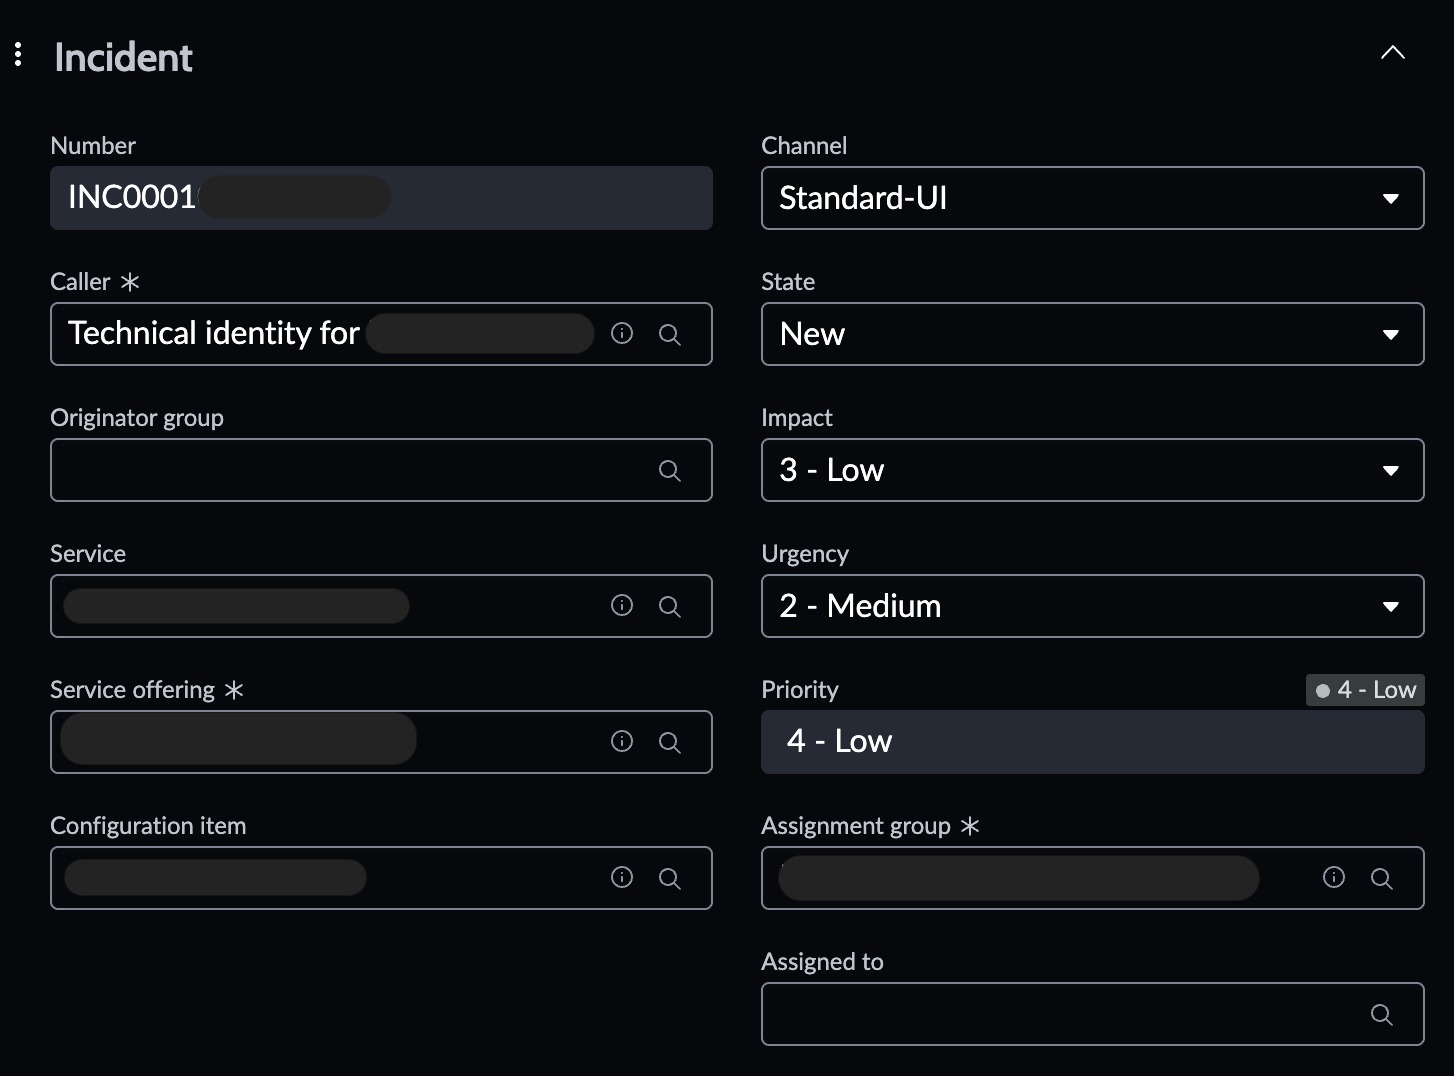
\includegraphics[width=\textwidth,keepaspectratio]{img/IncidentDetails}
	\caption[Detalhes do incidente]{Detalhes do incidente}
	\label{fig:incidentDetails}
\end{figure}

Associado a cada incidente, existe ainda um titulo, normalmente sucinto e objetivo, e uma descrição mais detalhada do problema. É nestes campos que o membro da equipa de suporta inicia a sua análise, sendo bastante importante conter descrições detalhadas, o que nem sempre é possível (Figura \ref{fig:incidentDescription}).

\begin{figure}[H]
\centering
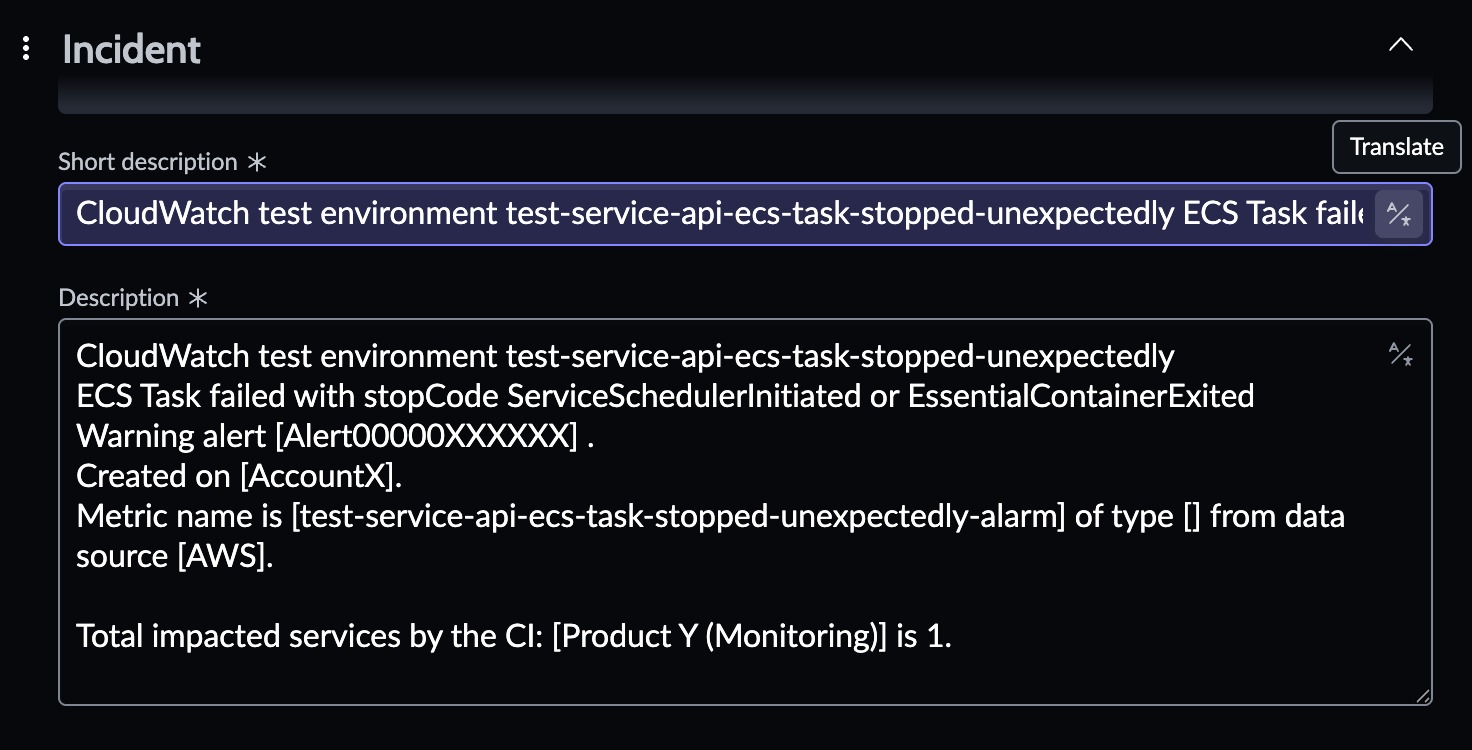
\includegraphics[width=\textwidth,keepaspectratio]{img/IncidentDescription}
\caption[Detalhes do incidente]{Detalhes do incidente}
\label{fig:incidentDescription}
\end{figure}

Para além dos campos originais do incidente, os desenvolvedores podem ainda deixar comentários extra que podem ser visíveis para o cliente ou apenas para as equipas de suporte. Esta abordagem é útil quando um incidente afeta várias equipas (Figura \ref{fig:incidentNotes}).

\begin{figure}[H]
\centering
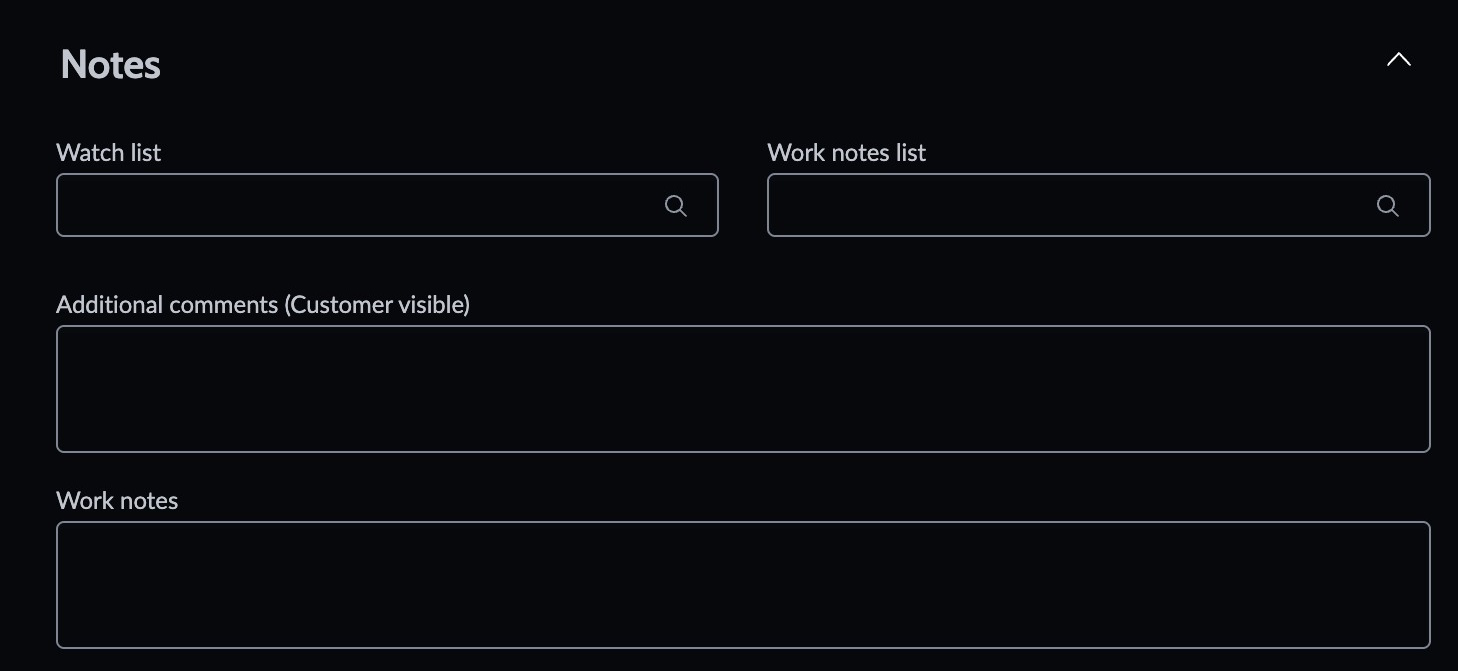
\includegraphics[width=\textwidth,keepaspectratio]{img/IncidentNotes}
\caption[Detalhes do incidente]{Detalhes do incidente}
\label{fig:incidentNotes}
\end{figure}

Por fim, o incidente precise de notas de resolução onde os \gls{OCEs} podem informar sobre os passos efetuados, origem do problema e outros comentários que achar necessário (Figura \ref{fig:incidentResolution}).

\begin{figure}[H]
\centering
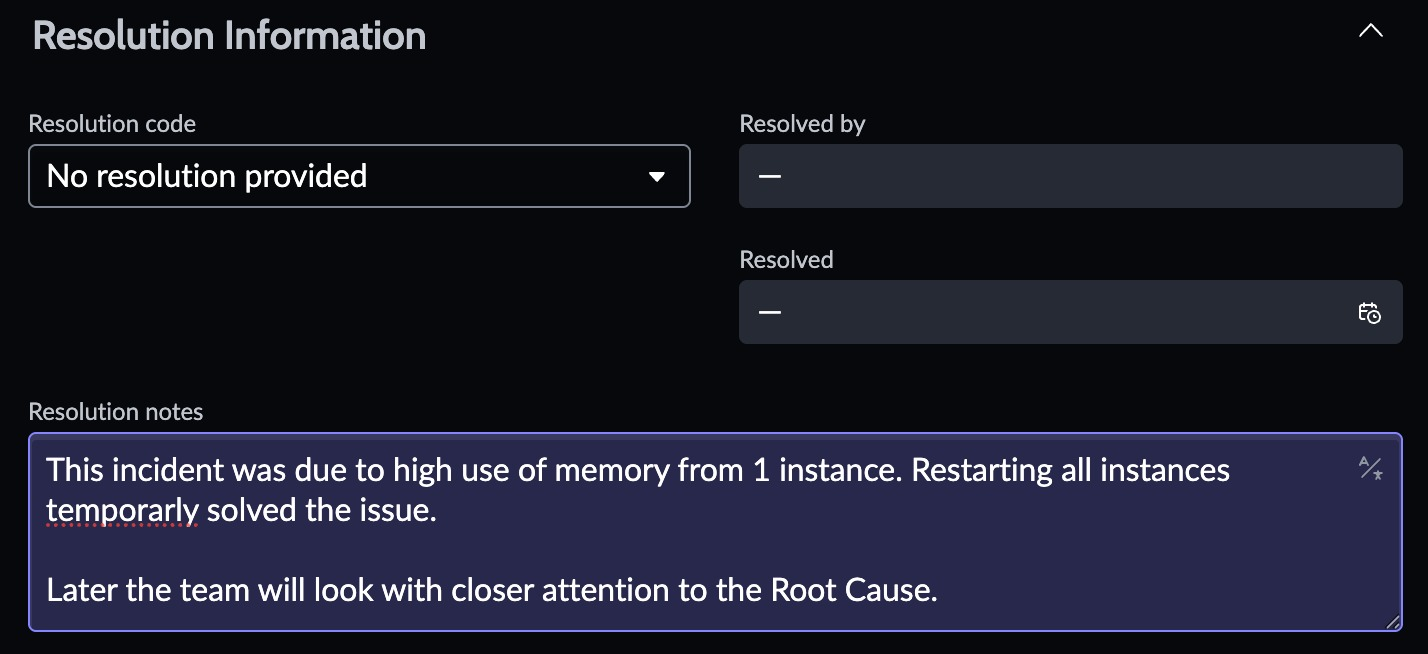
\includegraphics[width=\textwidth,keepaspectratio]{img/IncidentResolution}
\caption[Detalhes do incidente]{Detalhes do incidente}
\label{fig:incidentResolution}
\end{figure}